\documentclass{article}
\usepackage{inputenc}
\title{Applied Mathematics Course Report}
\author{Dejian, Li(11521046)}
\date{April 2016}

\usepackage{natbib}
\usepackage{graphics}
\usepackage{graphicx}		% import used as insert eps file
\usepackage{cite}			% import used as cite articles
\begin{document}
\maketitle
\begin{abstract}
	% Here we input the abstract part words
	In this work I detailed read the recommended article 《Very deep convolution networks for large scale image recognition》[1]. My main contribution is divided into three parts, a brief introduction of convolutions networks used in deep learning, applied LeNet structure in Caltech101 dataset, thorough analysis of VGG network along with the abstraction of status of very deep network cause limit of my current GPU computation ability.   
\end{abstract}
\section{Convolution Networks}
In the last few years, deep neural networks have lead to breakthrough results on a variety of computer vision problems. Specifically, one of the essential components named Convolution networks have recently achieved a huge success both in image annotation and object category classification. Intuitively, convolution neural network[2] can be thought of as a kind of composition of different neurons to propagate back and force to generate an understanding rule in a task. Suppose you are looking at an single digital number image (0-9) and you want to figure out which number is in that image. A typical way to do this recognition is set several neurons to represent different kinds of information a graphic could have, such as edge, color, background etc. Then simply connect them all together to a fully connected layer. However, this is too difficult to define an suitable single neuron to extract specific image features. An idea is to direct extract features and then using these features to represent image characters. Based on this idea, Sift[3] and HOG[4] are two of the most accepted hand-crafted methods, but these two methods still not performed very good since some of image information got lost during feature extraction. Therefore, a more sophisticated approach is to treat a whole image into  several local parts and create a stacked neurons to look image information again and again. This makes each layer of neurons only focus on one aspect of an image which matches attention about local properties of the image data. This means each layer will compute certain features, and one very nice property of convolutional layers is that they are composable, which means the output of one convolution layer can feed into another layer. Since the convolution operation will increase the number of original data, they are often interweaved with pooling layers, one popular pooling layer is called max-pooling layer that is zoom a pixel region to the biggest pixel value in this region. From a high level perspective, human don't care about the precise point in time a feature is present. 
\section{Implementation LeNet in Caltech101}
LeNet is a well-known convolution network that is widely used in different classification datasets. Especially in MNIST[4], LeNet had achieved high accuracy rate, and a lot of latter deeper CNN networks are adopted the idea of in building LeNet more or less. Therefore, I used LeNet-5 as basic network framework and adjusted some layers in order to get higher test rate in Caltech101. The main work can be divided in three steps. The first step is prepare training data, the second part is about build the network in caffe along with link all configuration together to train network, the final part is about methods adopted to increasing accuracy rate such fine-tuning and so on. The whole operation will under deep learning toolbox named Caffe[5].
\subsection{Prepare Data}
There are lots of data type that caffe accepts, detail definition can referred codes in data layer cpp file in caffe framework. Generally, Database(type: 'Data'), HDF5 Input(type: 'HDF5Data') and Images(type: 'ImageData') are three commonly used in recent researches. However, caffe it also support some other data type such as Windows Data, In-Memory Data and Dummy Data(under development and debugging). Because the file in Calthch101 database are original images file which already satisfy the data type in caffe, all needs to be done is create two text files respectly contain train images path and test(also can be called validation) images path. Then both these two files will feed into caffe network prototxt file to locate train images and test images in training phase and test phase respective. Specifically, each line in these two text files is defined with two parts divided with a blank, one part is absolute path to locate a specific image file and the other part is its category number. To create this kind of file can be either done in a shell script or python sys.path programming way. What's more, we also need to calculate the image mean binaryproto since each time caffe to solve its network will call on this file. One trick here is we can use mean binaryproto from other images which also gives us very good results. This can be illustrated that for general image processing, the mean value would changed a lot. By the way, we do not corp each image manually because caffe would done this job automatically. We made train images ten times larger than test images. After done these two steps and build the correct file we need, then we can move to build convolution layer part.
\subsection{Building Network In Caffe}
A normal LeNet contains 6 layers(show in figure 1). Because original LeNet was used in hand written digital recognition, there are only 10 classes that softmax dealt with. However, in Caltech101 dataset, the categories are 101, therefore, in the last full connected layer will output 101 units to softmax classifier to classify. Compared the size of MNIST dataset with Calthch101 dataset, Caltech101 dataset is about ten times larger than MNIST dataset. This underlies that to train the same network in Caltech101 needs at least 10 times more than in MNIST. And borrow ideas from VGG network which shows that 3$\times$3 convolution filter size is best in image recognition task. Based on those points, I designed three networks with original LeNet to figure out what kind of network will improve accuracy(show in figure 2).The difference between test1 and LeNet is we simply changed the convolutional kernel size from five to three. And for test2, we add one more stacked convolution layer to increase the depth of the network. For test3, we add a useful activation function called ReLU[6] in each convolutional layer. Furthermore, as a conclusion drew by Simonyan et.al[1], we also used AlexNet[6] to verify the deep network helps classification task(see figure 3)lexNet contains five convolution layer and two full connected layer which is much bigger than all four nets in the above.
\subsection{Training Process and Results}
	The test net training procedure generally follows LeNet. Because short of GPU resources, we use mini-batch method and the batch size was set to 20. The training was regularized by weight decay 5e-3, and the learning rate was initially set to $10^{-3}$. The learning rate would decrease by a factor of 10 when iteration equals to 1500. In total, the learning rate was decreased 3 times, and by the end of training the learning process didn't stopped. This means, we haven't did fine tuning in those net yet. 
	The initialization of the weights is important, since bad initialization can stall learning due to saturation of activation function. To circumvent this problem, we adopted Adam[7] methods and initialize weights by Xavier[8]. During the training time, we scale learning rate each 1500 iteration ten percent of itself. And this makes the whole net converges to a good results. The results are showed in following table(see table 1). Intuitively, the accuracy is increased by each net, this gives the result that each adjustment is positive to improve classification task. Furthermore, it can be see that the Test2 makes a huge improvement compared with LeNet, this gives a evidence that adjust network into deep network is actually helps. 
%在tabular 环境中,用& 跳入下一列,用\\ 开始新的一行,用\hline 插入 水平表线
\begin{table}
\centering
	\begin{tabular}[b!]{|c|c|c|c|c|c|c|}
	\hline
	Net. & 1000 & 2000 & 3000 & 4000 & 5000 & acc\\
	\hline
	LeNet & 49.3\% & 50.3\% & 51.1\% & 51.3\% & 51.3\% & 51.3\% \\
	Test1 & 51.0\% & 52.8\% & 53.3\% & 53.6\% & 53.5\% & 53.6\% \\
	Test2 & 52.7\% & 54.4\% & 56.0\% & 55.4\% & 55.3\% & 56.8\% \\
	Test3 & 52.7\% & 58.9\% & 57.7\% & 58.2\% & 58.5\% & 58.9\% \\
	\hline
	\end{tabular}
\caption{Different network accuracy under different iterations}
\label{table:1}
\end{table}
\section{VGG Network}
In this part, based on the article 《Very deep convolution networks for large scale image recognition》[1]. I will introduce its network architecture, methods used to train and test data. Finally, a short discussion about whether deep network is better would also be mentioned. 
\subsection{Architecture}
During training, the input data is a fixed-size 224$\times$224 RGB image. Then use 3$\times$3 convolution filter with stride 1. Then feed it to 2$\times$2 max pooling filter with stride 2. The whole network can be seen as eight parts. Five stacked convolutional layers, each group has different configuration(A~E), two fully connected layer and one fully connected softmax classification layer(See table2). The key points in VGG stacked convolution network is it uses 3$\times$3 filter with stride 1 which was experimented to be the best filter size. And uses rectification unit to faster whole training process.
\begin{table}
% 下面这一个语句用于实现在表格内换行
\newcommand{\tabincell}[2]{\begin{tabular}{@{}#1@{}}#2\end{tabular}}
\centering
	\begin{tabular}{|c|c|c|c|c|}
	%\hline \multicolumn{5}{c}{ConvNet Configuration}\\
	\hline
		A & B & C & D & E \\
	\hline
		conv3-64 & \tabincell{c}{conv3-64 \\ LRN} & \tabincell{c}{conv3-64 \\ conv3-64} & \tabincell{c}{conv3-64 \\ conv3-64} & \tabincell{c}{conv3-64 \\ conv3-64}\\
	\hline
		conv3-128 & conv3-128 & \tabincell{c}{conv3-128 \\ conv3-128} & \tabincell{c}{conv3-128 \\ conv3-128} & \tabincell{c}{conv3-128 \\ conv3-128}\\
	\hline
		\tabincell{c}{conv3-256 \\ conv3-256} & \tabincell{c}{conv3-256 \\ conv3-256} & \tabincell{c}{conv3-256 \\ conv3-256 \\ conv1-256} & \tabincell{c}{conv3-256 \\ conv3-256 \\ conv3-256} & \tabincell{c}{conv3-256 \\ conv3-256 \\ conv3-256 \\ conv3-256}\\
	\hline
		\tabincell{c}{conv3-512 \\ conv3-512} & \tabincell{c}{conv3-512 \\ conv3-512} & \tabincell{c}{conv3-512 \\ conv3-512 \\ conv1-512} & \tabincell{c}{conv3-512 \\ conv3-512 \\ conv3-512} & \tabincell{c}{conv3-512 \\ conv3-512 \\ conv3-512 \\ conv3-512}\\
	\hline
		\tabincell{c}{conv3-512 \\ conv3-512} & \tabincell{c}{conv3-512 \\ conv3-512} & \tabincell{c}{conv3-512 \\ conv3-512 \\ conv1-512} & \tabincell{c}{conv3-512 \\ conv3-512 \\ conv3-512} & \tabincell{c}{conv3-512 \\ conv3-512 \\ conv3-512 \\ conv3-512}\\
	\hline \multicolumn{5}{c}{maxpool} \\
	\hline \multicolumn{5}{c}{FC-4096} \\
	\hline \multicolumn{5}{c}{FC-4096} \\
	\hline \multicolumn{5}{c}{FC-4096} \\
	\hline \multicolumn{5}{c}{soft-max} \\
	\hline
	\end{tabular}
\caption{VGG network configuration}
\label{Table:2}
\end{table}
\subsection{VGG Results}
The results of VGG net can be listed as follows.For training phase, it provides an extensive empirical for 16 or 19 layers trained on 384$\times$N images are the best training size and training scale jittering is better than fixed scales. That means if need 256 size data, we can use 512 size data to crop into several 256 size data slips to use as 256 size data. As for the ImageNet problems, VGG network performs the second place with 7.3\% and one single model has 8.4\% error(see figure5). All the results implied that the depths of network really matters in classification problem.
\subsection{Comments on Very deep network}
As a branch of machine learning, it seems once using deep learning whether audio, video or image recognition, the accuracy will automatically get a huge improvement without fine-tuning. In my opinion, one vital reason is that it matches a saying in the machine learning that is 'It's not who has the best algorithm that wins. It's who has the most data.'. This means the essential of building very deep network is to construct more data based on the input data and try to learn these data together. Followed by this idea, researches found it is worth while to build deeper and deeper networks and the trained model weights can use as initial weights in other similar network. That is, these networks have good quality of generalization which  also matches the biological facts of human brain, convex used in see area can also be used in listen area, both two area have capability of see and listen, the only cause them difference is that when signal transparent in our brain, it prefers to separate different signals and sent them to different parts of human brain to parallelism processing. Followed by this idea, we applied AlexNet in caltech101 and fine tuning the last layer(fc8, classification layer), the results is impressive, in the meanwhile, even without fine tuning version also achieved quite good results(see figure 6 and 7).However, there also some difficulties remaining to explore. Sophisticate network bring more parameters which needs lots of computer resources during training process, and this challenges researchers to come up with faster training methods as well as to avoid overfitting problems. 
\section{Acknowledgments}
This work was supported by csmath class. I gratefully acknowledge the support of senior laboratory Super Lee with the donation of the GPU used for this work. \newline \newline
\begin{figure}[b!]
	\centering
	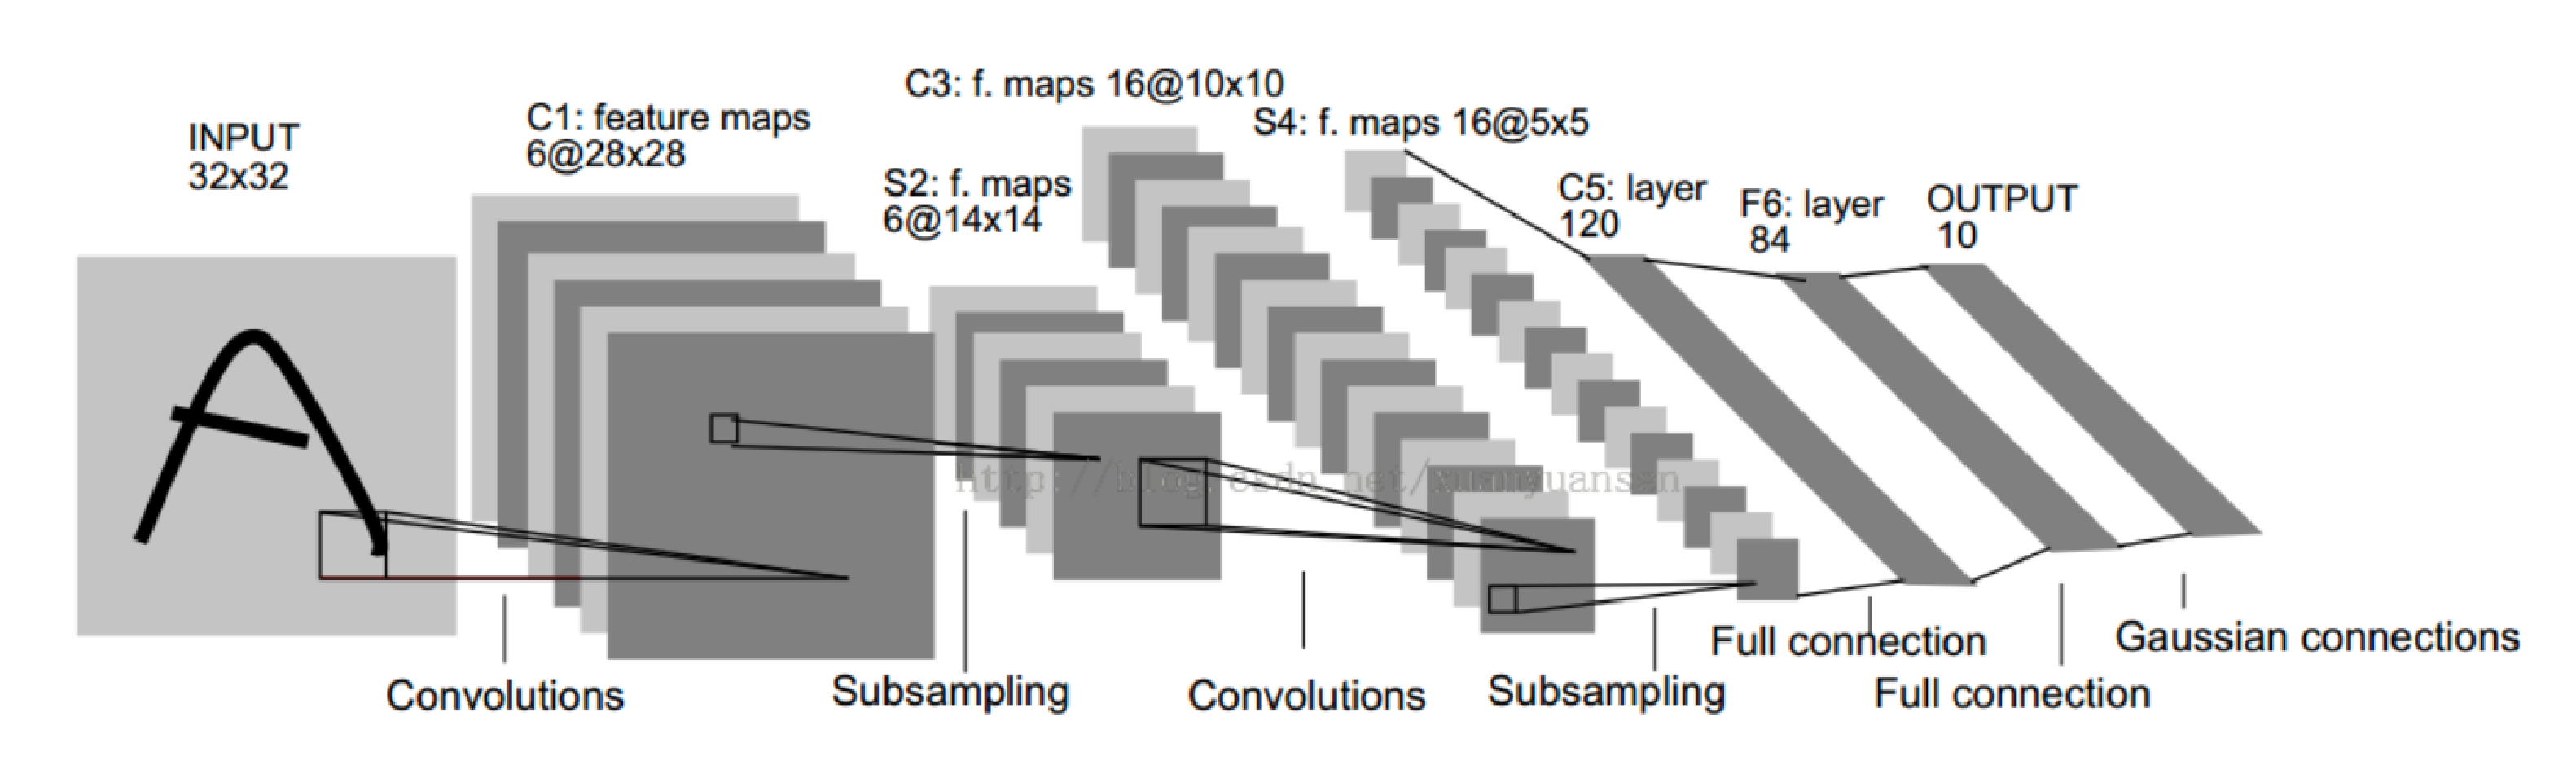
\includegraphics[width=0.9\columnwidth]{figure_1}
	\caption{Architecture of LeNet-5, a Convolutional Neural Network, here for digits recognition. Each plane is a feature map, i.e. a set of units whose weights are constrained to be identical.}
	\label{fig:1}
\end{figure}
\begin{figure}
	\centering
	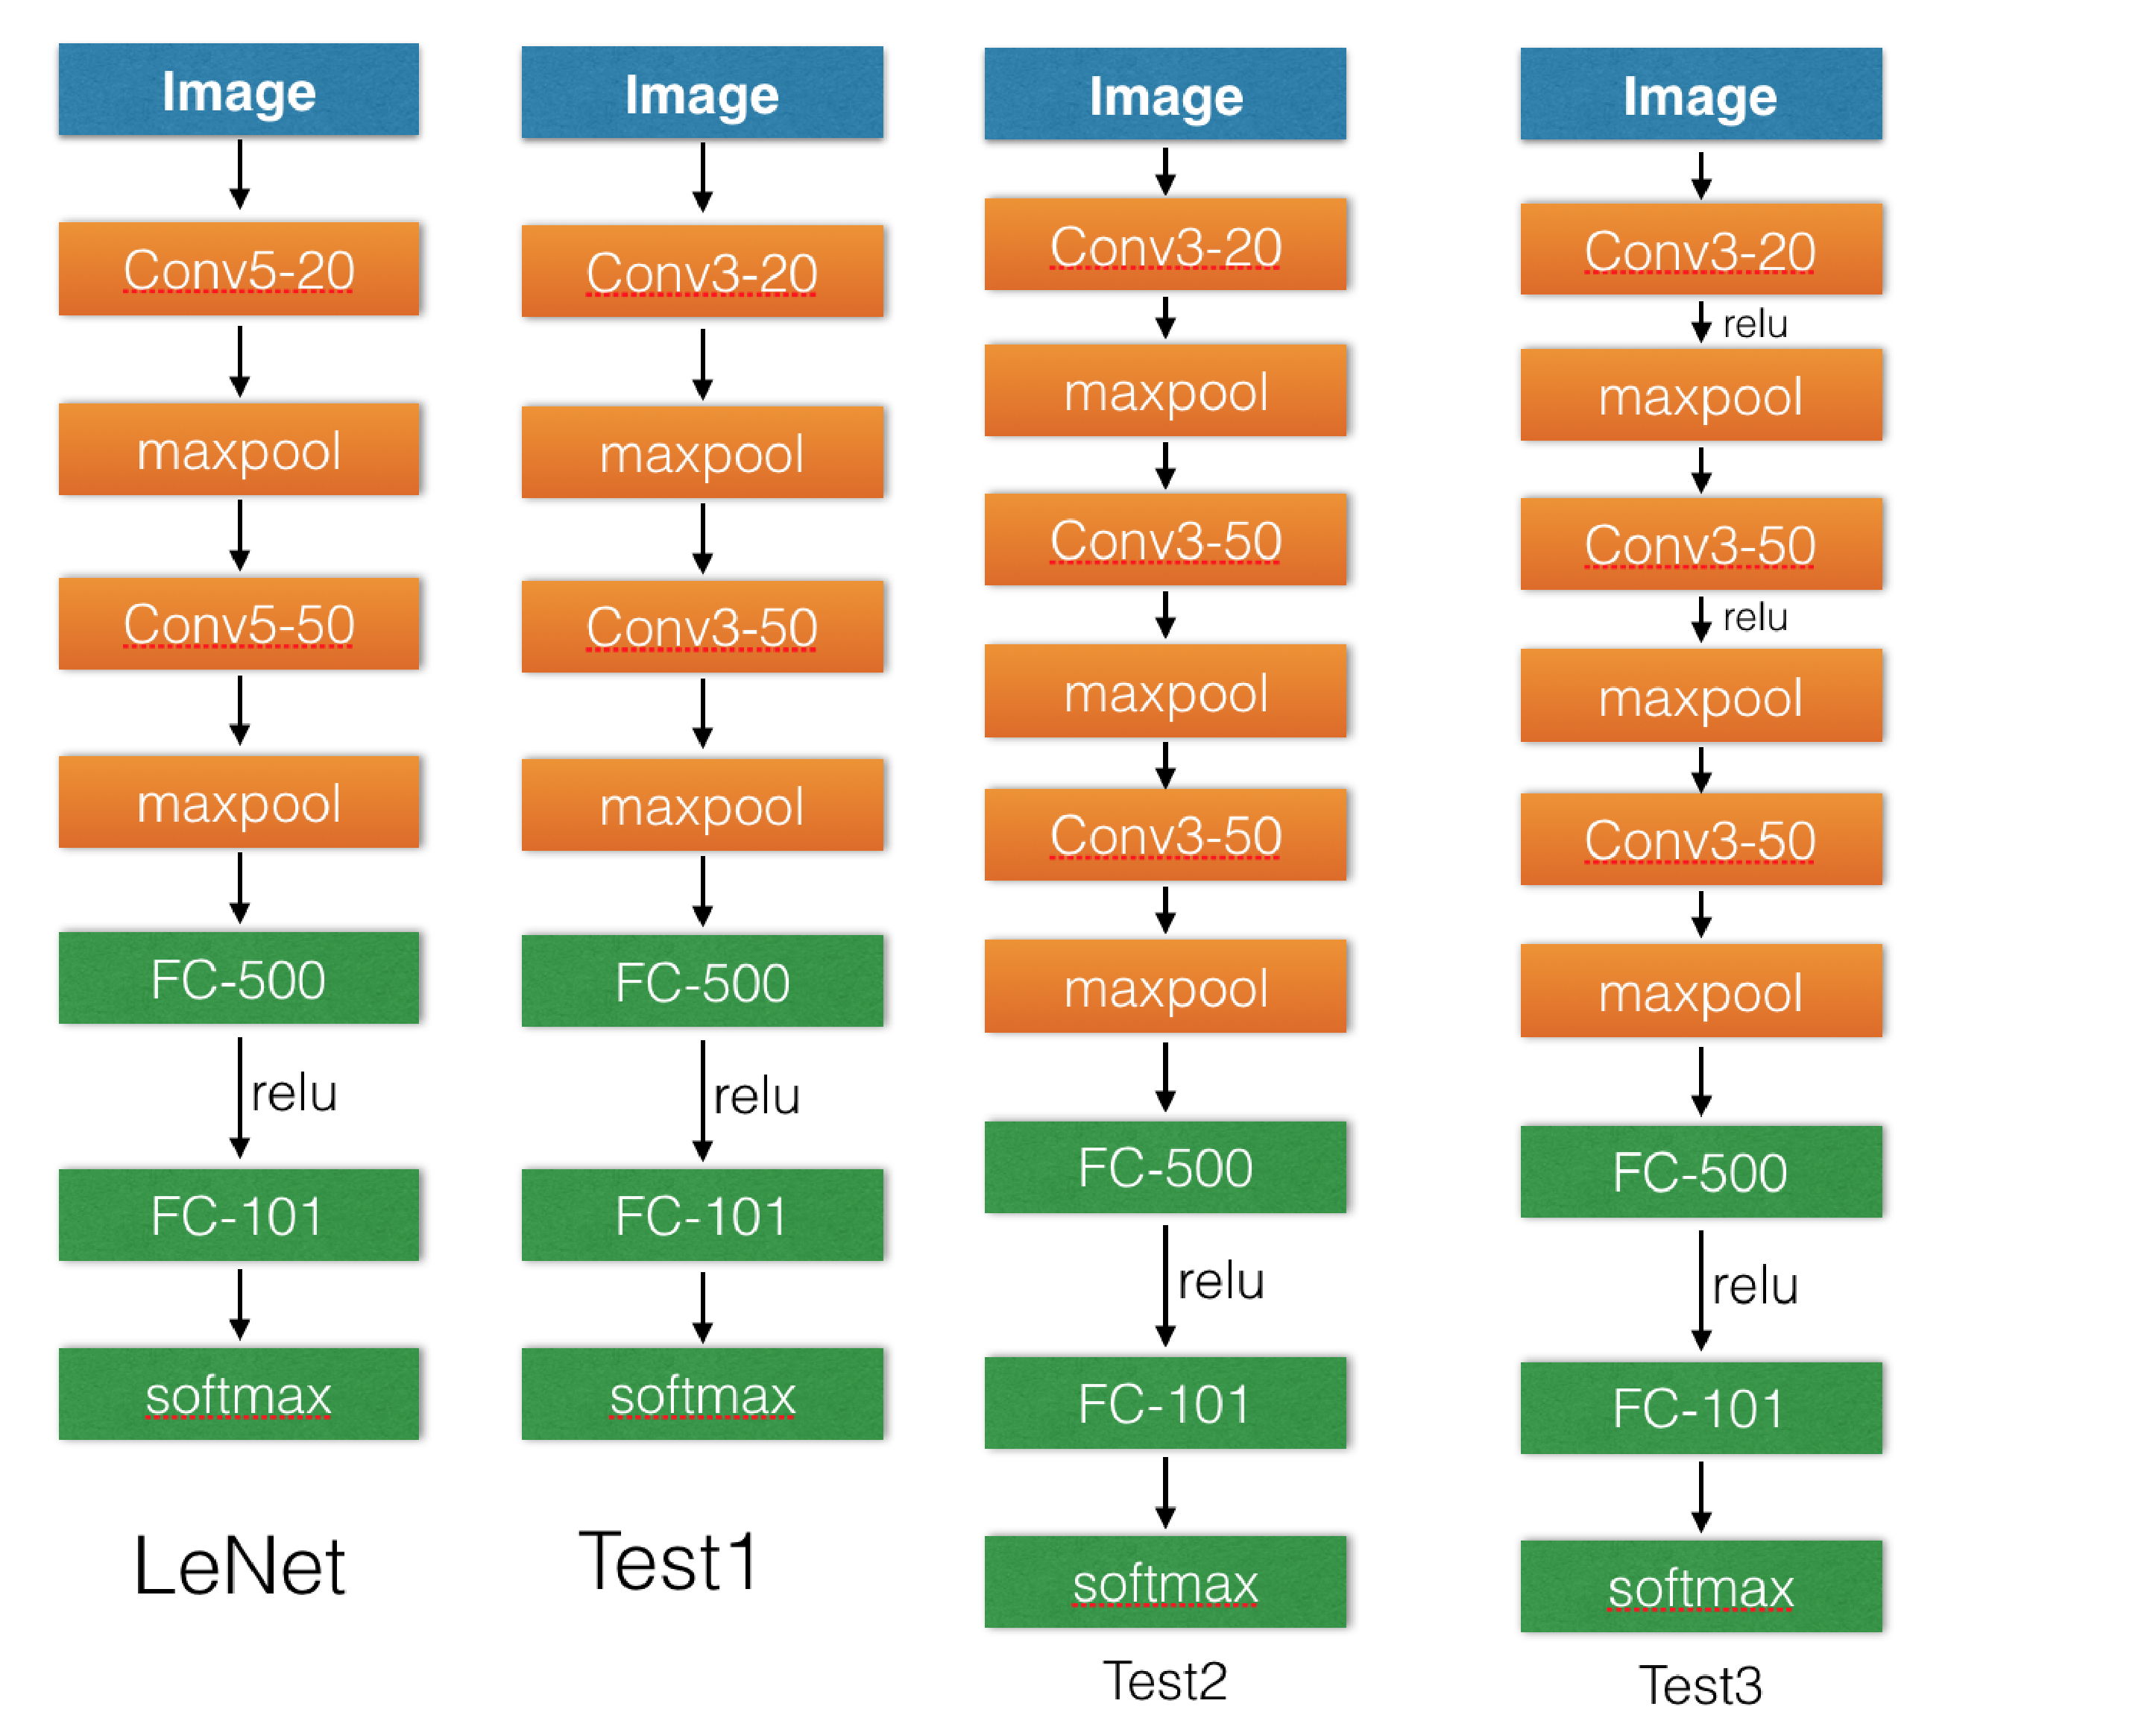
\includegraphics[width=0.9\columnwidth]{test_net}
	\caption{Four different networks}
	\label{fig:2}
\end{figure}
\begin{figure}[b!]
	\centering
	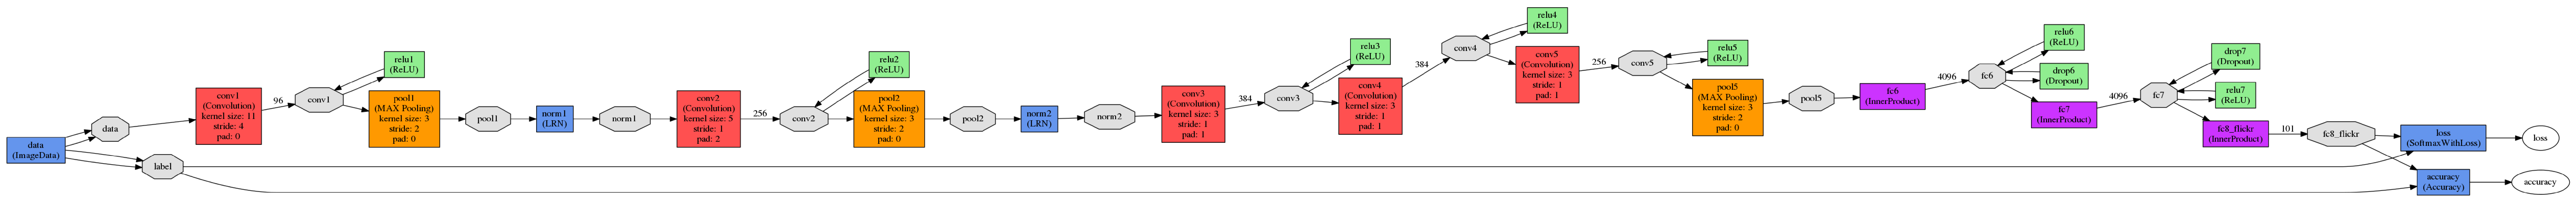
\includegraphics[width=0.9\columnwidth]{deepnet}
	\caption{The AlexNet, we adjust the last layer fc8 output unit 20 into 101}
	\label{fig:3}
\end{figure}
\begin{figure}
	\centering
	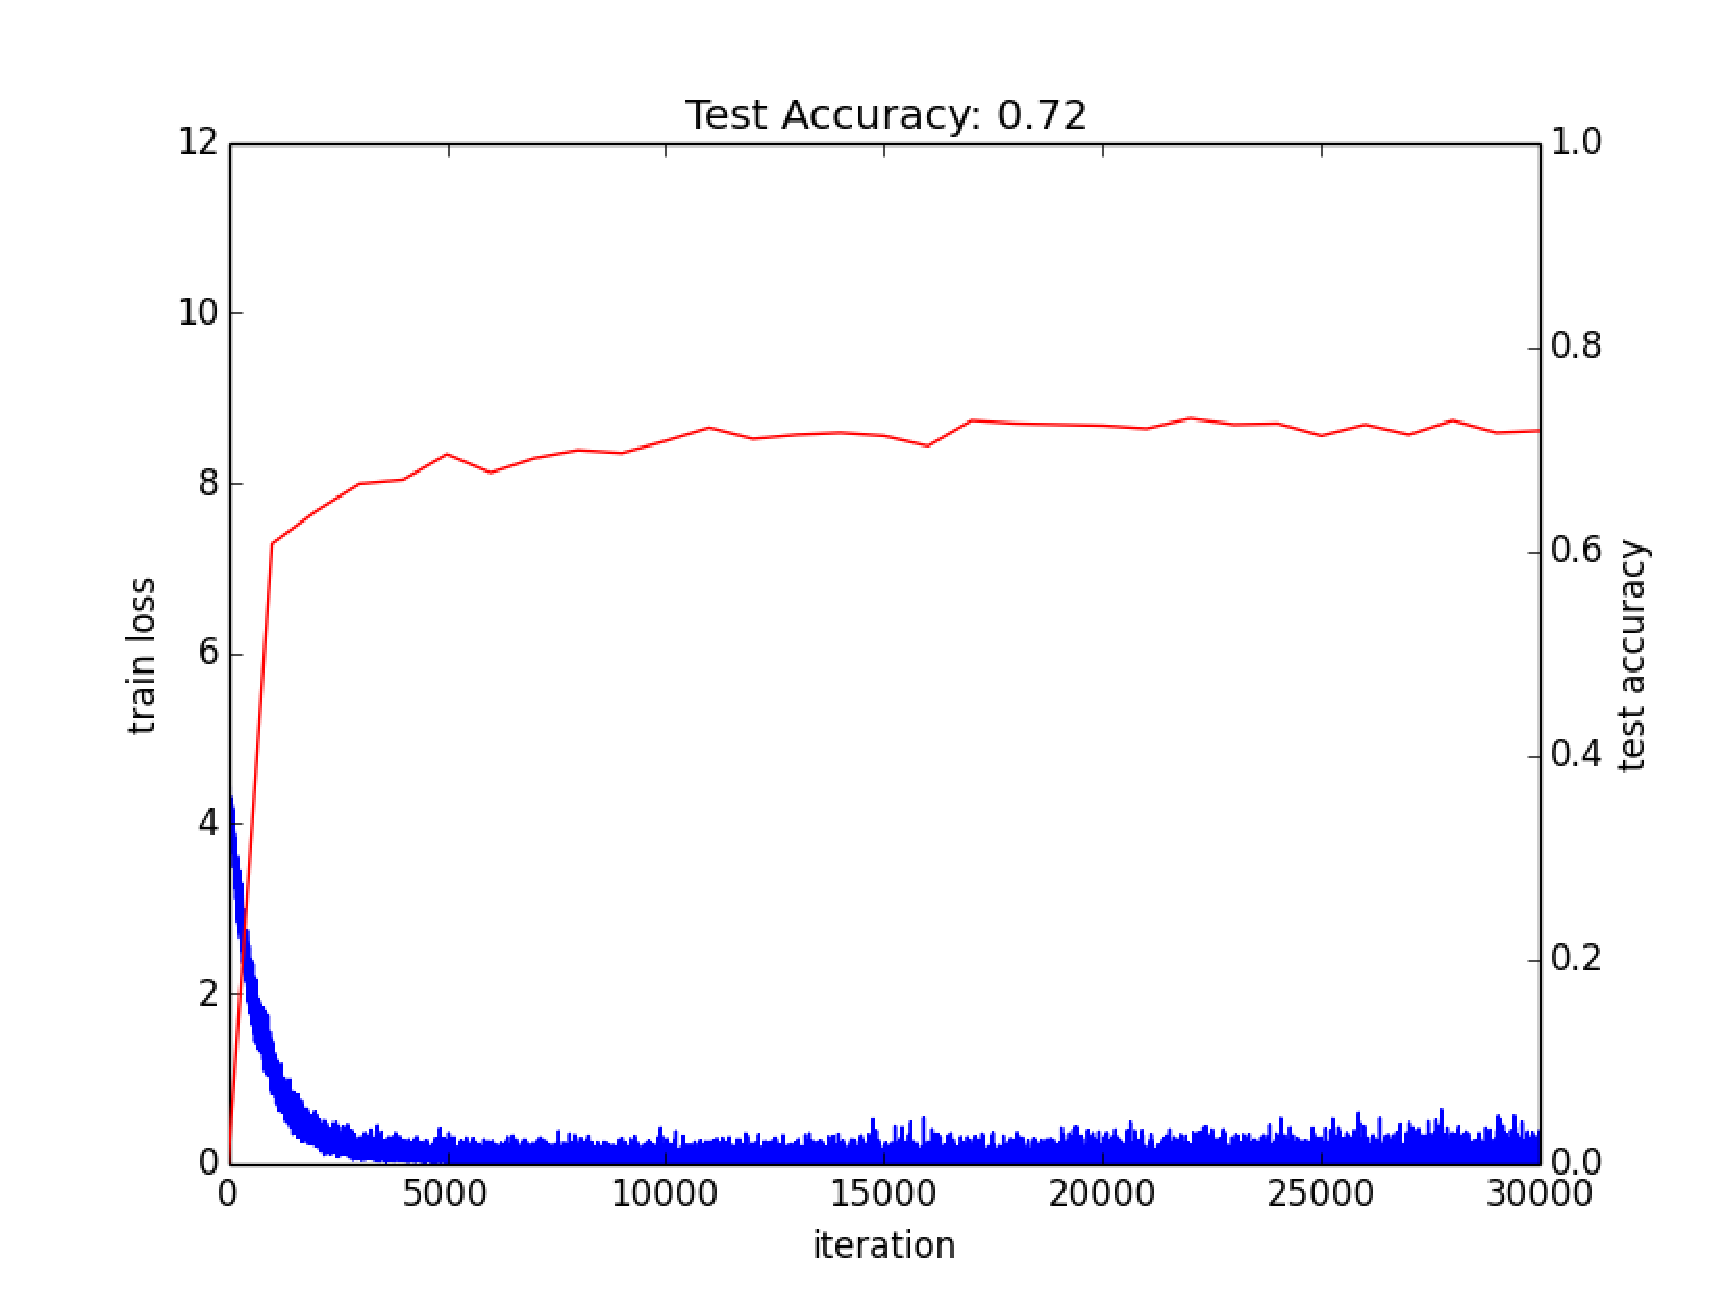
\includegraphics[width=0.9\columnwidth]{depnet1}
	\caption{see}
	\label{fig:4}
\end{figure}
\begin{figure}[b!]
	\centering
	% much easier way to scale size, just got the rate between width picture and with page
	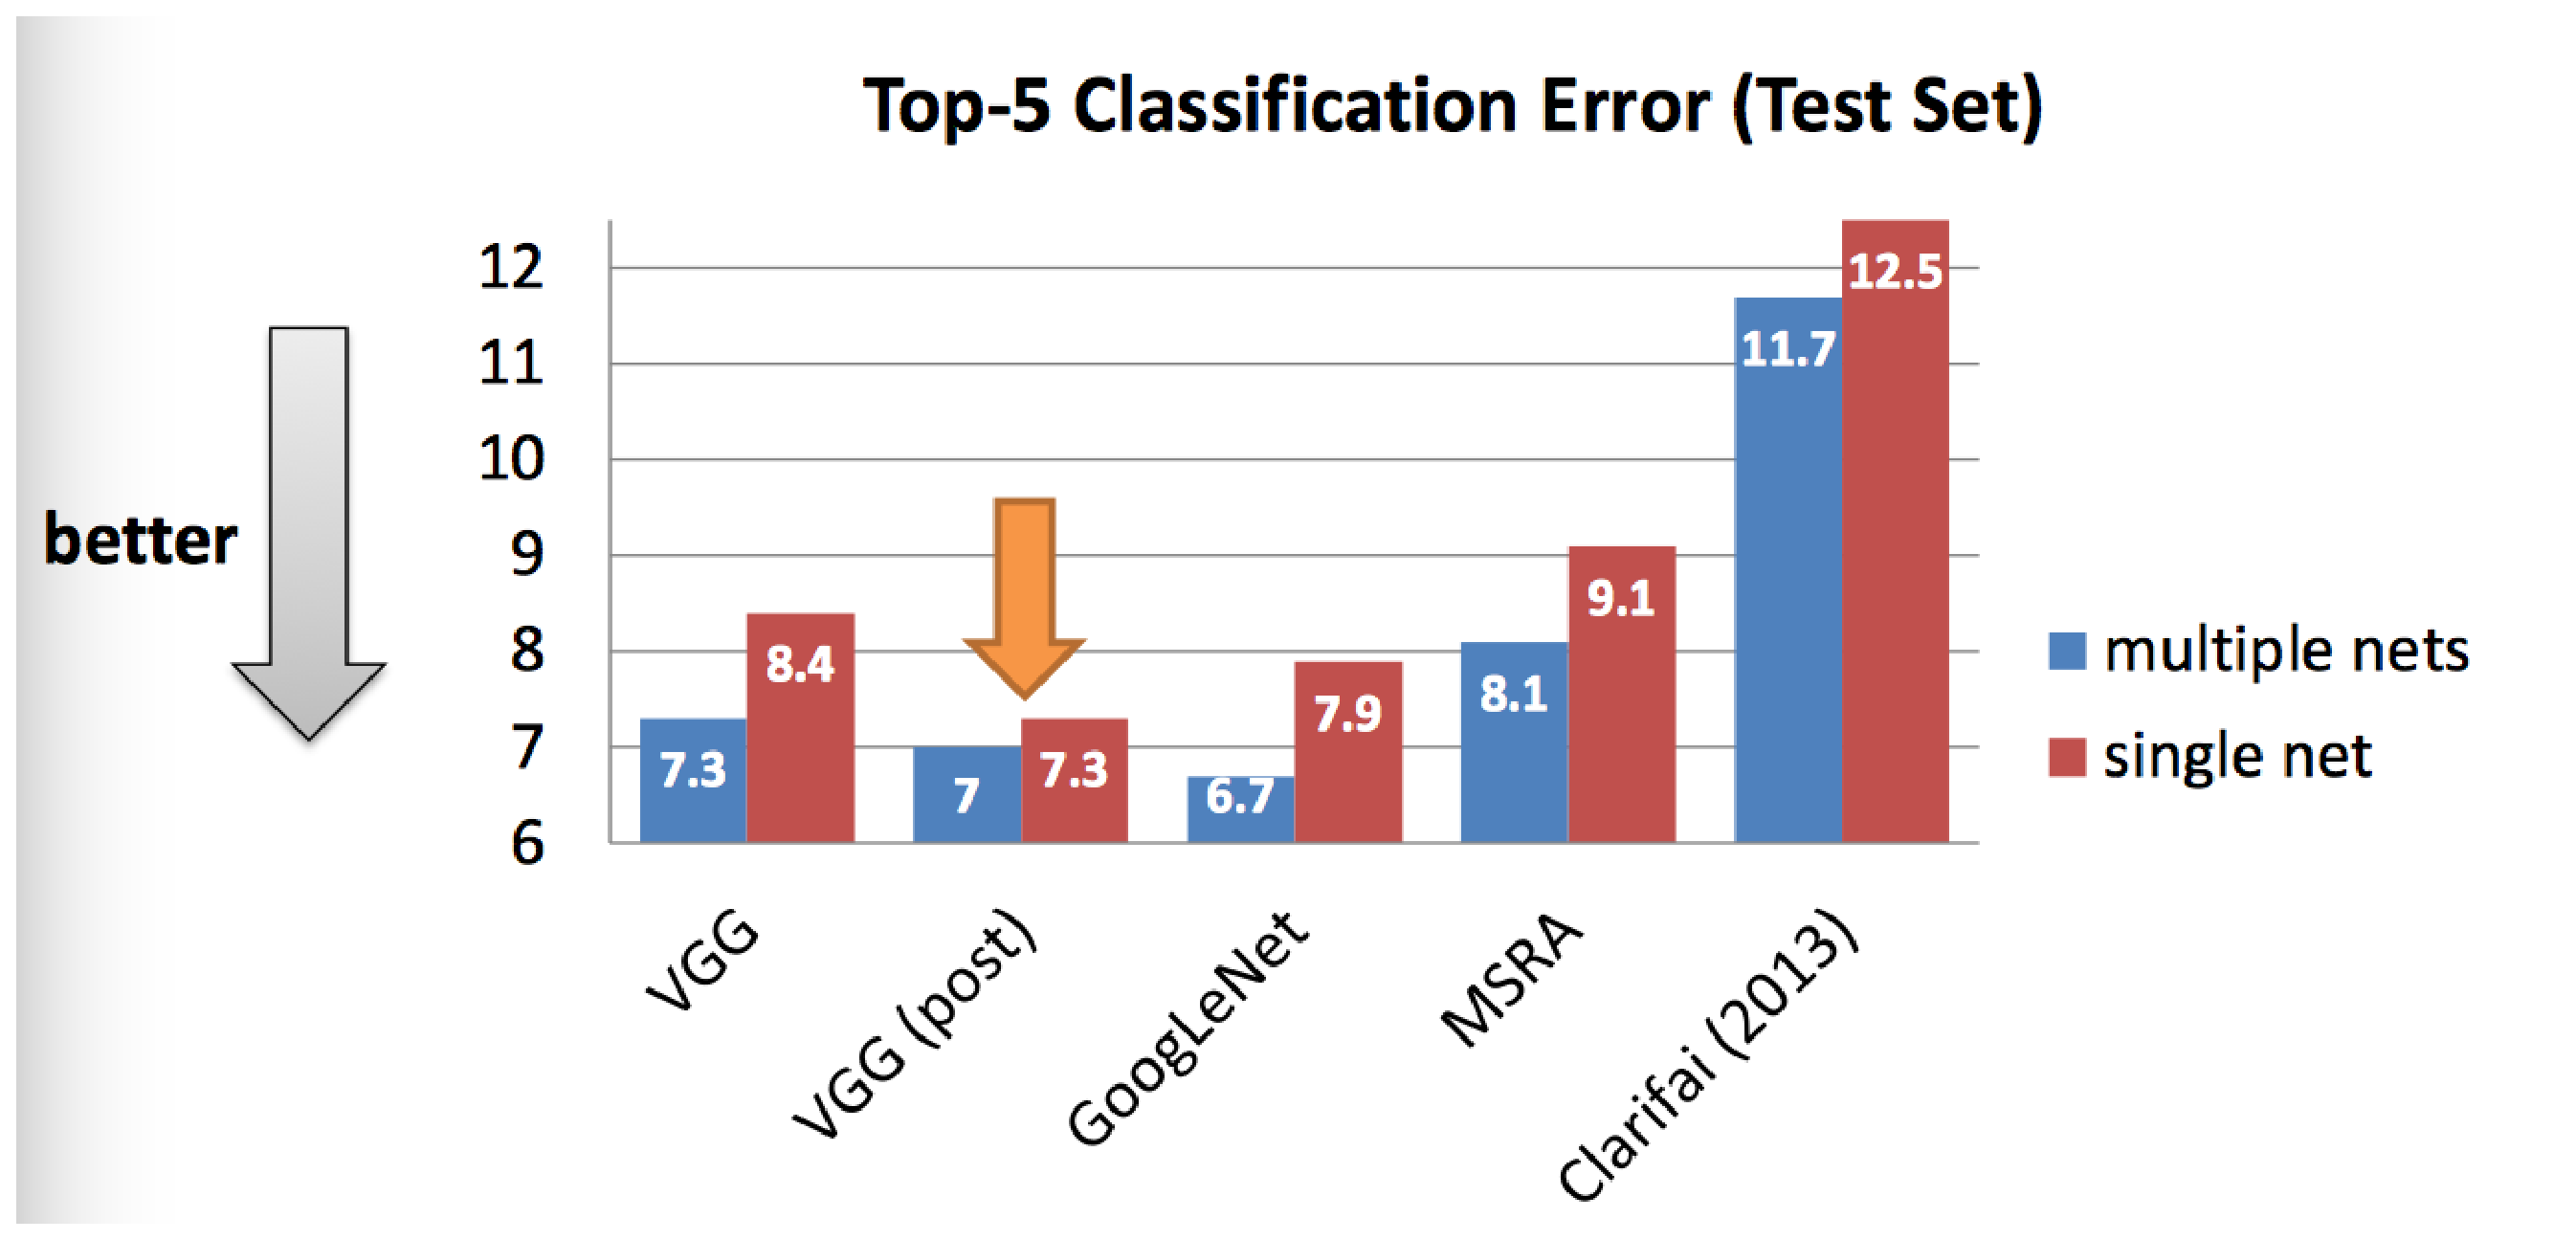
\includegraphics[width=0.9\columnwidth]{figure_2}
	\caption{Results of AlexNet}
	\label{fig:5}
\end{figure}
\begin{figure}[b!]
	\centering
	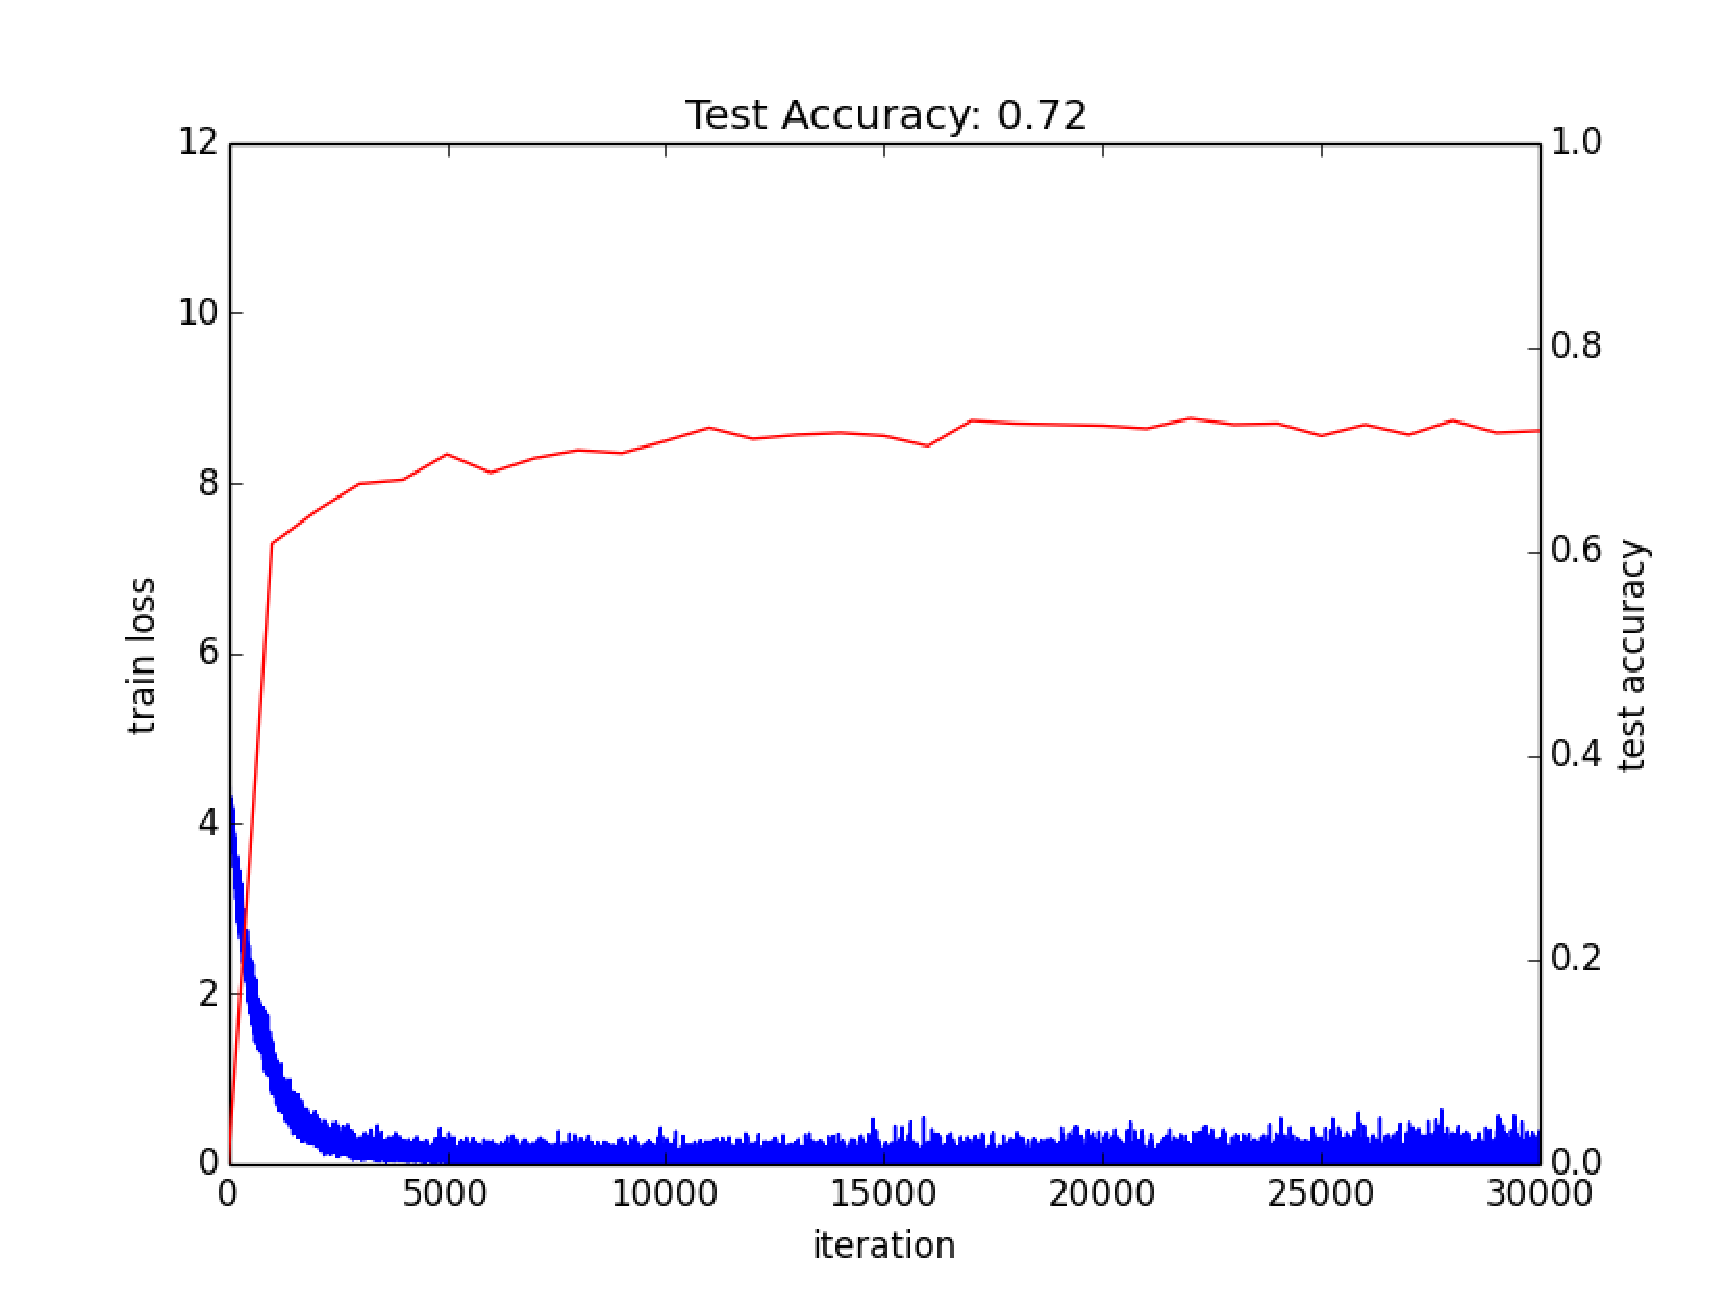
\includegraphics[width=0.9\columnwidth]{depnet1}
	\caption{AlexNet without Fine tuning}
	\label{fig:6}
\end{figure}
\begin{figure}
	\centering
	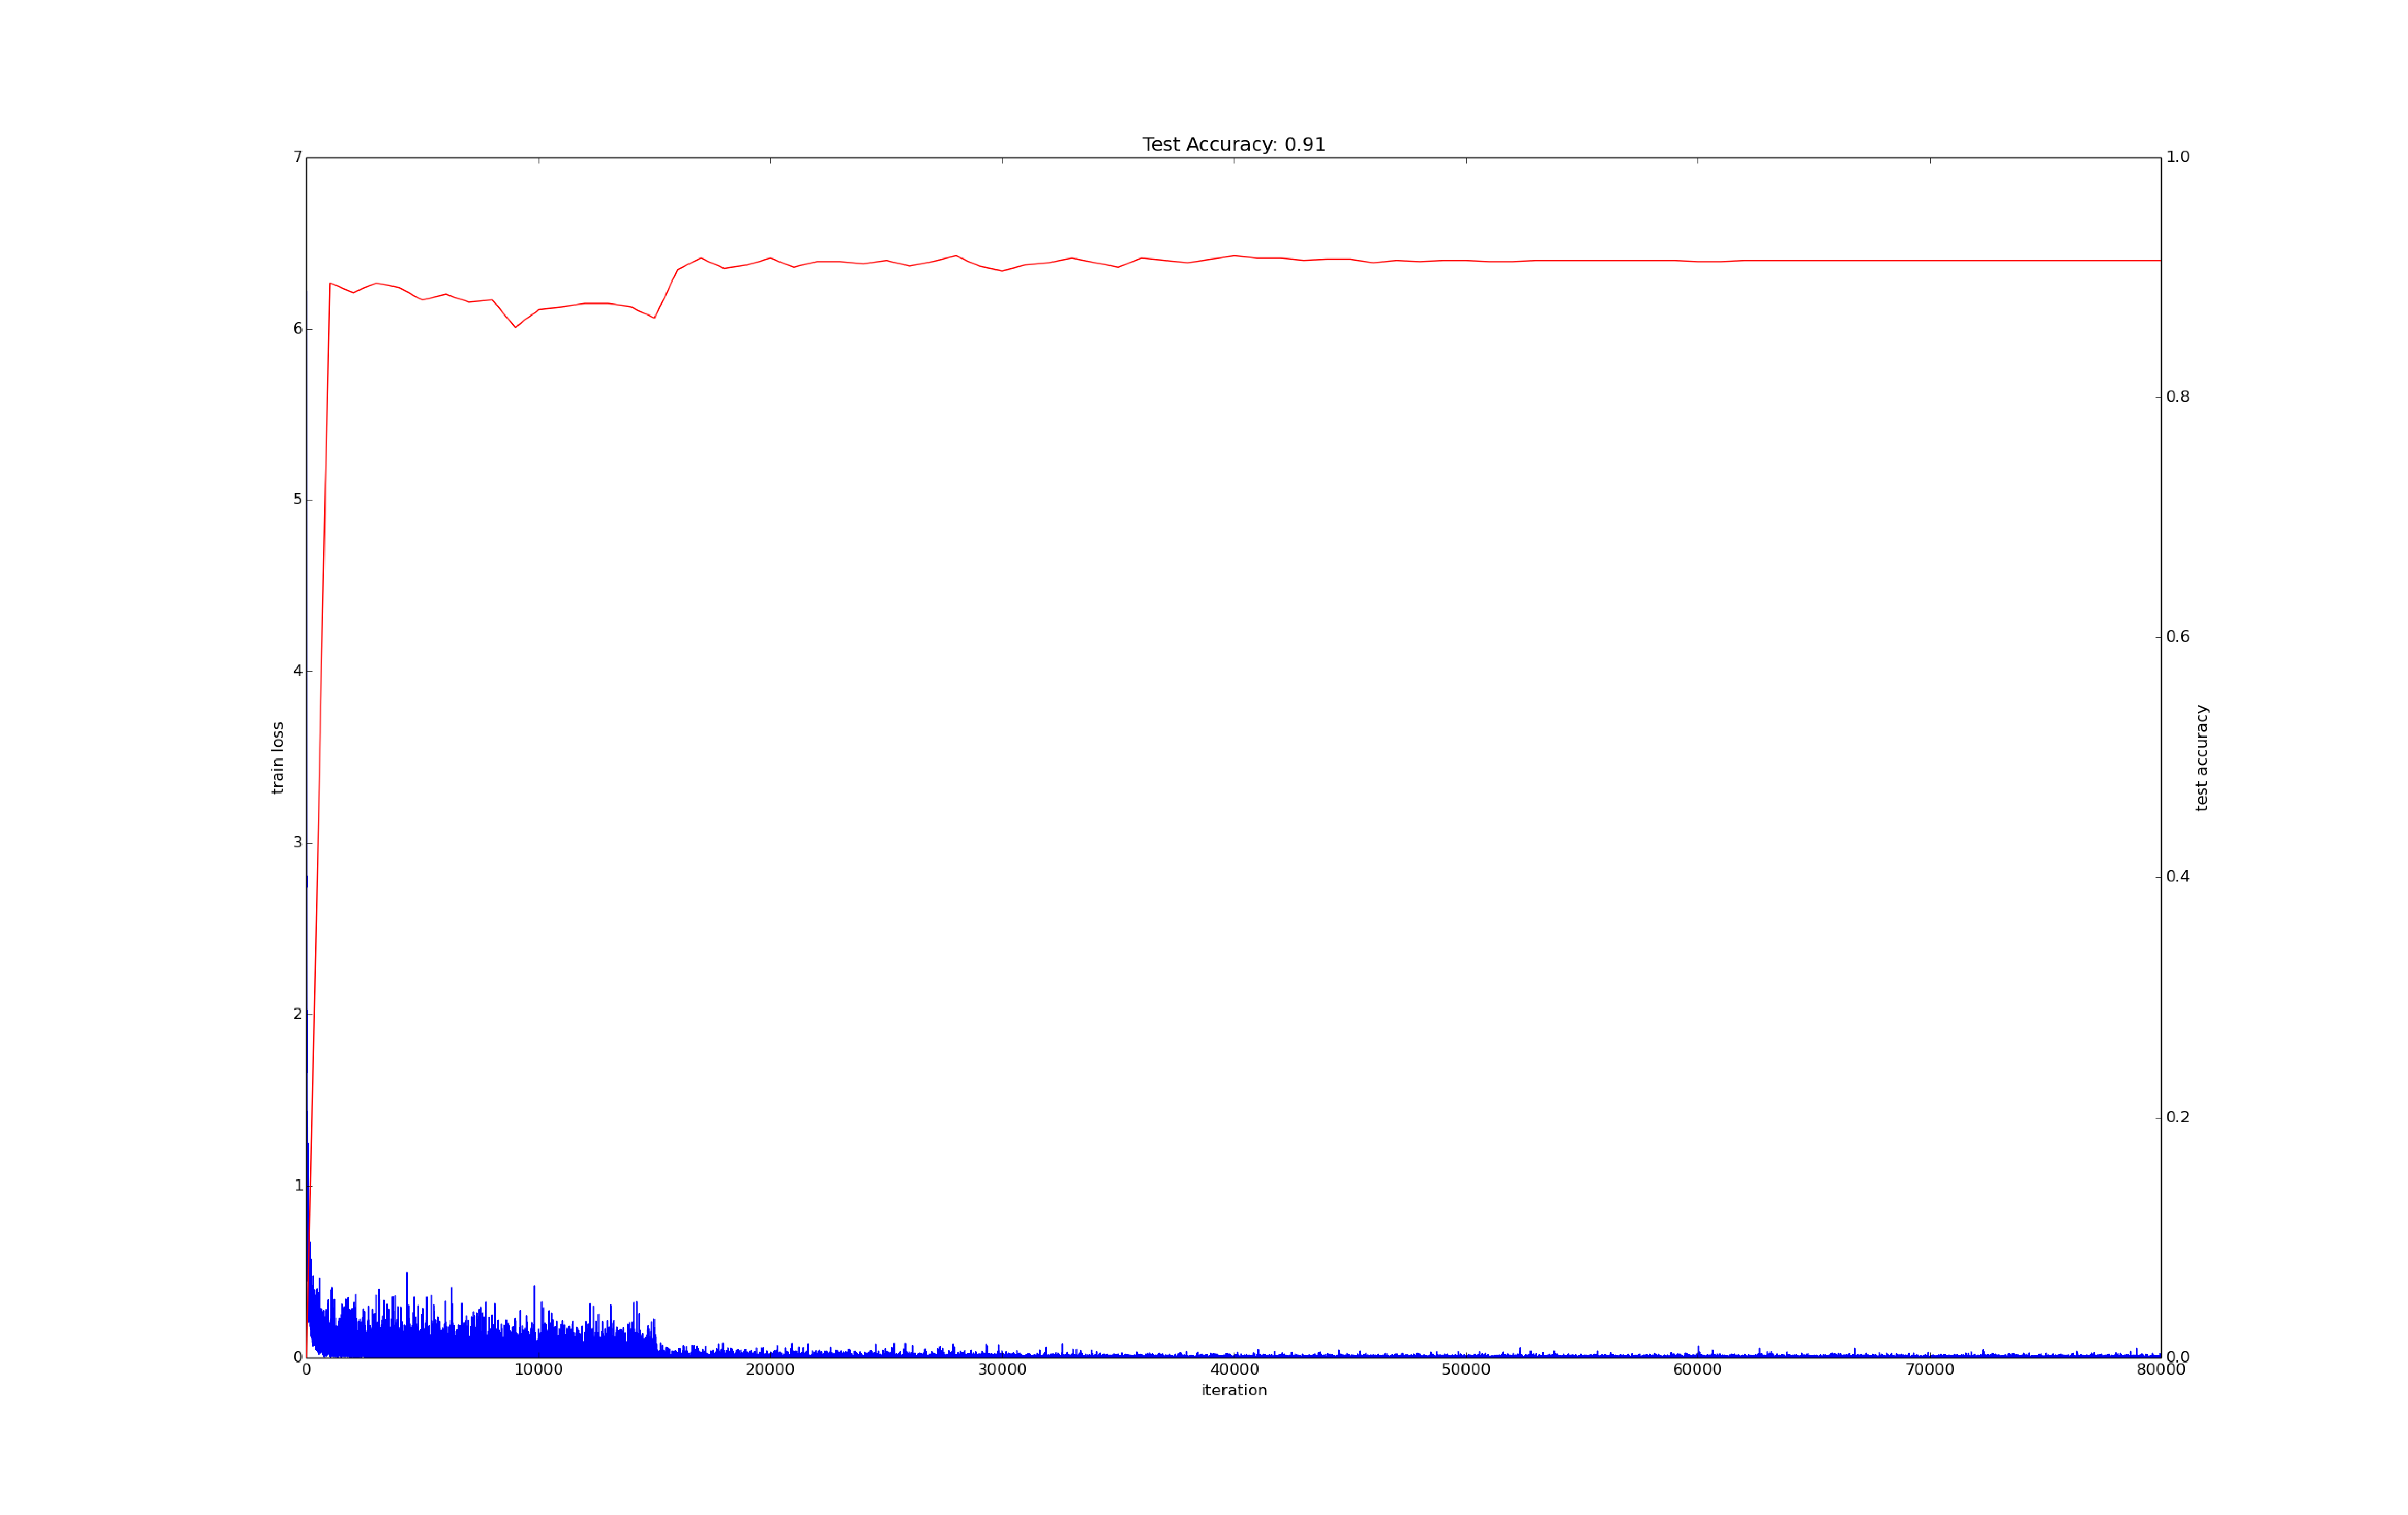
\includegraphics[width=0.9\columnwidth]{final_f1}
	\caption{AlexNet with Fine tuning}
	\label{fig:7}
\end{figure}
\section{Reference} 
[1] Simonyan K, Zisserman A. Very deep convolutional networks for large-scale image recognition[J]. arXiv preprint arXiv:1409.1556, 2014. \newline
[2] LeCun Y, Bengio Y. Convolutional networks for images, speech, and time series[J]. The handbook of brain theory and neural networks, 1995, 3361(10): 1995. \newline
[3] Ke Y, Sukthankar R. PCA-SIFT: A more distinctive representation for local image descriptors[C]//Computer Vision and Pattern Recognition, 2004. CVPR 2004. Proceedings of the 2004 IEEE Computer Society Conference on. IEEE, 2004, 2: II-506-II-513 Vol. 2. \newline
[4] Dalal N, Triggs B. Histograms of oriented gradients for human detection[C]//Computer Vision and Pattern Recognition, 2005. CVPR 2005. IEEE Computer Society Conference on. IEEE, 2005, 1: 886-893. \newline
[5] Jia Y, Shelhamer E, Donahue J, et al. Caffe: Convolutional architecture for fast feature embedding[C]//Proceedings of the ACM International Conference on Multimedia. ACM, 2014: 675-678. \newline
[6] Krizhevsky A, Sutskever I, Hinton G E. Imagenet classification with deep convolutional neural networks[C]//Advances in neural information processing systems. 2012: 1097-1105. \newline
[7] Kingma D, Ba J. Adam: A method for stochastic optimization[J]. arXiv preprint arXiv:1412.6980, 2014. \newline
[8] Glorot X, Bengio Y. Understanding the difficulty of training deep feedforward neural networks[C]//International conference on artificial intelligence and statistics. 2010: 249-256. \newline
\end{document}